\documentclass[serif,xcolor=pdftex,dvipsnames,table,hyperref={bookmarks=false,breaklinks}]{beamer}

%%%%%%%%%%%%%%%%
% Change the macros below to configure the title slides
% for your course.
\newcommand{\coursename}{COMPSCI 589}
\newcommand{\instructor}{Benjamin M. Marlin}
\newcommand{\university}{University of Massachusetts Amherst}
\newcommand{\department}{College of Information and Computer Sciences}
%%%%%%%%%%%%%%%%


\newcommand{\settitlecard}[2]{
  \title[\coursename  Lecture #1] 
    {\coursename \\ Lecture #1: #2}
     \author[\instructor]{\instructor}
     \institute[\university]{
     \department\\
     \university
   }
\date{}
}

\newcommand{\maketitlepage}{
  \begin{frame}
  \titlepage
  \center{
    %If you use the slides unmodified, retain the attribution below
    \tiny{Slides by Benjamin M. Marlin (marlin@cs.umass.edu). \\
    \vspace{-1em}Created with support from National Science Foundation Award\# IIS-1350522. 
    %If you modify the slides, please retain the alternate attribution below
    %\tiny{Based on slides by Benjamin M. Marlin (marlin@cs.umass.edu). \\    
    %\vspace{-1em}Created with support from National Science Foundation Award\# IIS-1350522. 
    }                                              
  }  
  \end{frame}
}

\AtBeginSection[]
{
  \begin{frame}<beamer>{Outline}
    \tableofcontents[currentsection,subsectionstyle=hide]
  \end{frame}
}


\newcommand{\cut}[1]{}

\newcommand{\iconbox}[4]{
  \only<#1-#2>{
    \begin{columns}[T]
      \column{0.5in}
           \includegraphics[width=0.5in]{#3}
       \column{3.7in}
            #4
    \end{columns}
    \medskip
    \medskip
    \medskip
  }
}

\mode<presentation>{
  \usepackage{../beamertheme589theme}
  \setbeamercovered{invisible}
}

\mode<handout>{
  \usepackage{../beamertheme589theme}
  \setbeamercovered{transparent}
}


\usepackage[english]{babel}
\usepackage[latin1]{inputenc}
\usepackage{times}
\usepackage[T1]{fontenc}
\usepackage{amsmath}
\usepackage{amssymb}
\usepackage[noend]{algorithmic}
\usepackage{algorithm}
\usepackage{listings}

\renewcommand\mathfamilydefault{\rmdefault}

\newcommand{\setA}{\mathcal{A}}
\newcommand{\setB}{\mathcal{B}}
\newcommand{\setS}{\mathcal{S}}
\newcommand{\setV}{\mathcal{V}}
\DeclareMathOperator*{\union}{\bigcup}
\DeclareMathOperator*{\intersection}{\bigcap}
\DeclareMathOperator*{\Val}{Val}
\newcommand{\mbf}[1]{{\mathbf{#1}}}
\DeclareMathOperator*{\argmax}{arg\,max}
\DeclareMathOperator*{\argmin}{arg\,min}
\DeclareMathOperator*{\sign}{sign}
\newcommand{\deriv}[2]{\frac{\partial{#1}}{\partial{#2}}}


\settitlecard{13}{Introduction to Apache Spark}

\begin{document}

\maketitlepage

\section{Review}
\subsection{foo}

\begin{frame}[t]{Moore's Law}
\center
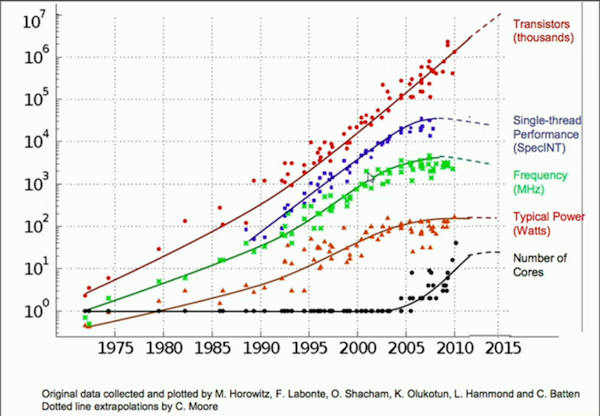
\includegraphics[width=3.5in]{../Figures/moores_law.png}\\[6pt]

Machine Learning's free ride ended in about 2005.
\end{frame}

\begin{frame}[t]{Big Data}
\center
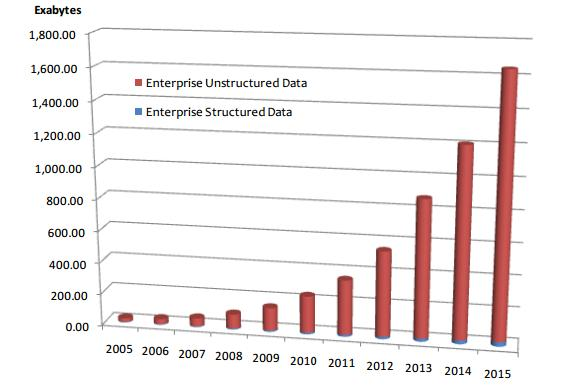
\includegraphics[width=3.5in]{../Figures/big_data.jpg}\\[6pt]

The amount of data is doubling every two years. 
\end{frame}

\begin{frame}[t]{Amdahl's Law}
\center
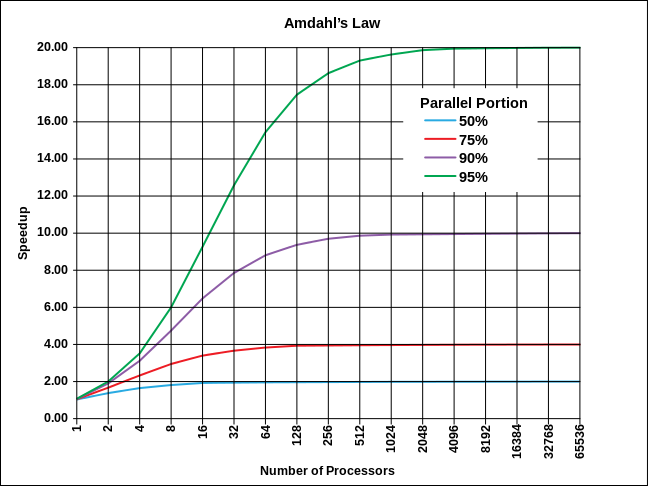
\includegraphics[width=3.5in]{../Figures/AmdahlsLaw.png}\\
\end{frame}

\begin{frame}[t]{Functional Programming and Data Parallel Computing}
\begin{itemize}
\item Functional programming is a natural match for data parallel computing
where we want to do things like:

\begin{itemize}
\pause \item Apply the same function to all elements in a 
data set (Map) 
\pause \item Apply a Boolean filter to select only certain data elements 
(Filter)
\pause \item Aggregate a number of data elements by summing, maxing, etc. 
(Reduce or Fold).
\end{itemize}

\pause \item It turns out that a small number of such easily parallelizable 
functional programming primitives are sufficient for creating data-parallel
implementations of machine learning algorithms. 

\end{itemize}
\end{frame}

\section{MapReduce}
\subsection{Foo}

\begin{frame}[t]{MapReduce and Hadoop}
\begin{itemize}

\item MapReduce is a distributed programming model 
introduced by Google in the early 2000's where all you can do is apply map and 
reduce functions to data. 

\pause\item Hadoop is a widely used open-source implementation of this 
framework.

\pause\item A scheduler breaks up the map 
computations over a cluster with a data-parallel distributed file system. The 
results of the map step are written back to the file system.

\pause\item The scheduler then schedules the reduce jobs on the cluster, which 
produce the final output and write it to the file system. 

\pause\item MapReduce uses a 
specialization of reduce for key-value pairs called \textit{reduce-by-key}.

\end{itemize}
\end{frame}


\begin{frame}[t]{Limitations of MapReduce For ML}
\begin{itemize}

\item The fact that MapReduce is completely stateless and all 
communication between processing iterations happens via the file system creates 
a significant synchronization barrier that negatively affects parallel 
scalability of iterative computations.

\pause
\center
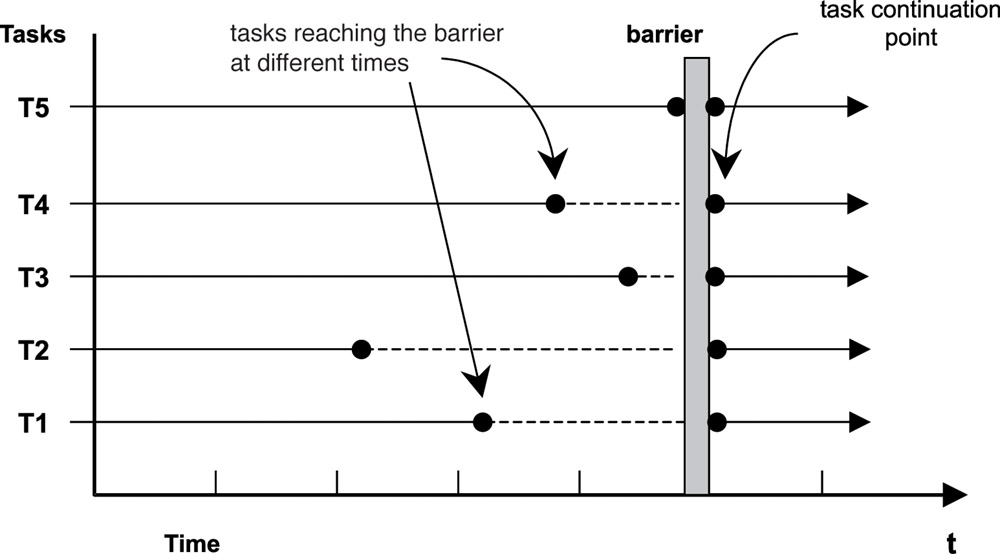
\includegraphics[width=3.4in]{../Figures/synchronization_barrier.jpg}\\

\end{itemize}
\end{frame}

\begin{frame}[t]{Apache Spark}
\begin{itemize}

\item Apache Spark is a parallel and distributed programming framework that 
adds additional parallel abstractions and allows for distributed 
in-memory caching as well as distributed on-disk data access. This makes it 
much faster than MapReduce for ML tasks.

\pause
\center
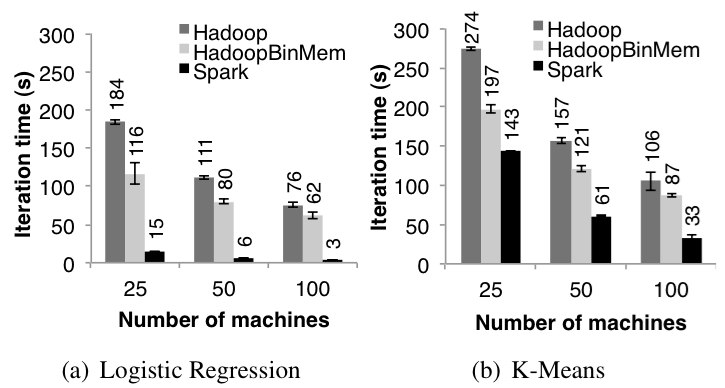
\includegraphics[width=3.4in]{../Figures/spark_vs_hadoop.png}\\
\end{itemize}

\end{frame}


\begin{frame}[t]{Apache Spark}

\center
\Huge Examples

\end{frame}

\end{document}
